\documentclass[]{article}
\usepackage{lmodern}
\usepackage{amssymb,amsmath}
\usepackage{ifxetex,ifluatex}
\usepackage{fixltx2e} % provides \textsubscript
\ifnum 0\ifxetex 1\fi\ifluatex 1\fi=0 % if pdftex
  \usepackage[T1]{fontenc}
  \usepackage[utf8]{inputenc}
\else % if luatex or xelatex
  \ifxetex
    \usepackage{mathspec}
  \else
    \usepackage{fontspec}
  \fi
  \defaultfontfeatures{Ligatures=TeX,Scale=MatchLowercase}
\fi
% use upquote if available, for straight quotes in verbatim environments
\IfFileExists{upquote.sty}{\usepackage{upquote}}{}
% use microtype if available
\IfFileExists{microtype.sty}{%
\usepackage{microtype}
\UseMicrotypeSet[protrusion]{basicmath} % disable protrusion for tt fonts
}{}
\usepackage[margin=1in]{geometry}
\usepackage{hyperref}
\hypersetup{unicode=true,
            pdftitle={post1},
            pdfauthor={Rongyun Tang},
            pdfborder={0 0 0},
            breaklinks=true}
\urlstyle{same}  % don't use monospace font for urls
\usepackage{color}
\usepackage{fancyvrb}
\newcommand{\VerbBar}{|}
\newcommand{\VERB}{\Verb[commandchars=\\\{\}]}
\DefineVerbatimEnvironment{Highlighting}{Verbatim}{commandchars=\\\{\}}
% Add ',fontsize=\small' for more characters per line
\usepackage{framed}
\definecolor{shadecolor}{RGB}{248,248,248}
\newenvironment{Shaded}{\begin{snugshade}}{\end{snugshade}}
\newcommand{\KeywordTok}[1]{\textcolor[rgb]{0.13,0.29,0.53}{\textbf{#1}}}
\newcommand{\DataTypeTok}[1]{\textcolor[rgb]{0.13,0.29,0.53}{#1}}
\newcommand{\DecValTok}[1]{\textcolor[rgb]{0.00,0.00,0.81}{#1}}
\newcommand{\BaseNTok}[1]{\textcolor[rgb]{0.00,0.00,0.81}{#1}}
\newcommand{\FloatTok}[1]{\textcolor[rgb]{0.00,0.00,0.81}{#1}}
\newcommand{\ConstantTok}[1]{\textcolor[rgb]{0.00,0.00,0.00}{#1}}
\newcommand{\CharTok}[1]{\textcolor[rgb]{0.31,0.60,0.02}{#1}}
\newcommand{\SpecialCharTok}[1]{\textcolor[rgb]{0.00,0.00,0.00}{#1}}
\newcommand{\StringTok}[1]{\textcolor[rgb]{0.31,0.60,0.02}{#1}}
\newcommand{\VerbatimStringTok}[1]{\textcolor[rgb]{0.31,0.60,0.02}{#1}}
\newcommand{\SpecialStringTok}[1]{\textcolor[rgb]{0.31,0.60,0.02}{#1}}
\newcommand{\ImportTok}[1]{#1}
\newcommand{\CommentTok}[1]{\textcolor[rgb]{0.56,0.35,0.01}{\textit{#1}}}
\newcommand{\DocumentationTok}[1]{\textcolor[rgb]{0.56,0.35,0.01}{\textbf{\textit{#1}}}}
\newcommand{\AnnotationTok}[1]{\textcolor[rgb]{0.56,0.35,0.01}{\textbf{\textit{#1}}}}
\newcommand{\CommentVarTok}[1]{\textcolor[rgb]{0.56,0.35,0.01}{\textbf{\textit{#1}}}}
\newcommand{\OtherTok}[1]{\textcolor[rgb]{0.56,0.35,0.01}{#1}}
\newcommand{\FunctionTok}[1]{\textcolor[rgb]{0.00,0.00,0.00}{#1}}
\newcommand{\VariableTok}[1]{\textcolor[rgb]{0.00,0.00,0.00}{#1}}
\newcommand{\ControlFlowTok}[1]{\textcolor[rgb]{0.13,0.29,0.53}{\textbf{#1}}}
\newcommand{\OperatorTok}[1]{\textcolor[rgb]{0.81,0.36,0.00}{\textbf{#1}}}
\newcommand{\BuiltInTok}[1]{#1}
\newcommand{\ExtensionTok}[1]{#1}
\newcommand{\PreprocessorTok}[1]{\textcolor[rgb]{0.56,0.35,0.01}{\textit{#1}}}
\newcommand{\AttributeTok}[1]{\textcolor[rgb]{0.77,0.63,0.00}{#1}}
\newcommand{\RegionMarkerTok}[1]{#1}
\newcommand{\InformationTok}[1]{\textcolor[rgb]{0.56,0.35,0.01}{\textbf{\textit{#1}}}}
\newcommand{\WarningTok}[1]{\textcolor[rgb]{0.56,0.35,0.01}{\textbf{\textit{#1}}}}
\newcommand{\AlertTok}[1]{\textcolor[rgb]{0.94,0.16,0.16}{#1}}
\newcommand{\ErrorTok}[1]{\textcolor[rgb]{0.64,0.00,0.00}{\textbf{#1}}}
\newcommand{\NormalTok}[1]{#1}
\usepackage{graphicx,grffile}
\makeatletter
\def\maxwidth{\ifdim\Gin@nat@width>\linewidth\linewidth\else\Gin@nat@width\fi}
\def\maxheight{\ifdim\Gin@nat@height>\textheight\textheight\else\Gin@nat@height\fi}
\makeatother
% Scale images if necessary, so that they will not overflow the page
% margins by default, and it is still possible to overwrite the defaults
% using explicit options in \includegraphics[width, height, ...]{}
\setkeys{Gin}{width=\maxwidth,height=\maxheight,keepaspectratio}
\IfFileExists{parskip.sty}{%
\usepackage{parskip}
}{% else
\setlength{\parindent}{0pt}
\setlength{\parskip}{6pt plus 2pt minus 1pt}
}
\setlength{\emergencystretch}{3em}  % prevent overfull lines
\providecommand{\tightlist}{%
  \setlength{\itemsep}{0pt}\setlength{\parskip}{0pt}}
\setcounter{secnumdepth}{0}
% Redefines (sub)paragraphs to behave more like sections
\ifx\paragraph\undefined\else
\let\oldparagraph\paragraph
\renewcommand{\paragraph}[1]{\oldparagraph{#1}\mbox{}}
\fi
\ifx\subparagraph\undefined\else
\let\oldsubparagraph\subparagraph
\renewcommand{\subparagraph}[1]{\oldsubparagraph{#1}\mbox{}}
\fi

%%% Use protect on footnotes to avoid problems with footnotes in titles
\let\rmarkdownfootnote\footnote%
\def\footnote{\protect\rmarkdownfootnote}

%%% Change title format to be more compact
\usepackage{titling}

% Create subtitle command for use in maketitle
\newcommand{\subtitle}[1]{
  \posttitle{
    \begin{center}\large#1\end{center}
    }
}

\setlength{\droptitle}{-2em}

  \title{post1}
    \pretitle{\vspace{\droptitle}\centering\huge}
  \posttitle{\par}
    \author{Rongyun Tang}
    \preauthor{\centering\large\emph}
  \postauthor{\par}
      \predate{\centering\large\emph}
  \postdate{\par}
    \date{December 11, 2018}


\begin{document}
\maketitle

\subsection{Census income}\label{census-income}

research outlines:

\begin{enumerate}
\def\labelenumi{\arabic{enumi}.}
\item
  Objective:task is to determine what kind of a person makes over 50K a
  year based on census data.
\item
  Method: statistics and association rules
\item
  Data Source: this ``Adult'' dataset was downloaded from UCI Machine
  Learning website: \url{http://archive.ics.uci.edu/ml/datasets/Adult}.
  It is multivariated dataset(including categorical and Integer
  variables) from social area. A set of reasonably clean records was
  extracted by the data dornors.It is also splited into train-test using
  MLC++ GenCVFiles (2/3, 1/3 random).
\end{enumerate}

=======================================================================================================

Attribute Information:

=======================================================================================================
Listing of attributes: salaries are potentially divided into two
classes: \textgreater{}50K, \textless{}=50K.

age: continuous. workclass: Private, Self-emp-not-inc, Self-emp-inc,
Federal-gov, Local-gov, State-gov, Without-pay, Never-worked. fnlwgt:
continuous. education: Bachelors, Some-college, 11th, HS-grad,
Prof-school, Assoc-acdm, Assoc-voc, 9th, 7th-8th, 12th, Masters,
1st-4th, 10th, Doctorate, 5th-6th, Preschool. education-num: continuous.
marital-status: Married-civ-spouse, Divorced, Never-married, Separated,
Widowed, Married-spouse-absent, Married-AF-spouse. occupation:
Tech-support, Craft-repair, Other-service, Sales, Exec-managerial,
Prof-specialty, Handlers-cleaners, Machine-op-inspct, Adm-clerical,
Farming-fishing, Transport-moving, Priv-house-serv, Protective-serv,
Armed-Forces. relationship: Wife, Own-child, Husband, Not-in-family,
Other-relative, Unmarried. race: White, Asian-Pac-Islander,
Amer-Indian-Eskimo, Other, Black. sex: Female, Male. capital-gain:
continuous. capital-loss: continuous. hours-per-week: continuous.
native-country: United-States, Cambodia, England, Puerto-Rico, Canada,
Germany, Outlying-US(Guam-USVI-etc), India, Japan, Greece, South, China,
Cuba, Iran, Honduras, Philippines, Italy, Poland, Jamaica, Vietnam,
Mexico, Portugal, Ireland, France, Dominican-Republic, Laos, Ecuador,
Taiwan, Haiti, Columbia, Hungary, Guatemala, Nicaragua, Scotland,
Thailand, Yugoslavia, El-Salvador, Trinadad\&Tobago, Peru, Hong,
Holand-Netherlands.

\begin{Shaded}
\begin{Highlighting}[]
\NormalTok{## 1. Data preprocessing}
\NormalTok{training.data <-}\StringTok{ }\KeywordTok{as.data.frame}\NormalTok{(}\KeywordTok{read.csv}\NormalTok{(}\StringTok{'adult.data'}\NormalTok{))}
\NormalTok{test.data <-}\StringTok{ }\KeywordTok{as.data.frame}\NormalTok{(}\KeywordTok{read.csv}\NormalTok{(}\StringTok{'adult.test'}\NormalTok{, }\DataTypeTok{skip=}\DecValTok{1}\NormalTok{))}
\NormalTok{content <-}\StringTok{ }\KeywordTok{readLines}\NormalTok{(}\StringTok{'old.adult.names'}\NormalTok{)}

\NormalTok{i <-}\StringTok{ }\KeywordTok{grep}\NormalTok{(}\StringTok{"Attribute Information"}\NormalTok{,content) }\OperatorTok{+}\StringTok{ }\DecValTok{2}
\NormalTok{  var.names <-}\StringTok{ }\OtherTok{NULL}
  \ControlFlowTok{while}\NormalTok{(content[i]}\OperatorTok{!=}\StringTok{""}\NormalTok{) \{}
\NormalTok{    j <-}\StringTok{ }\KeywordTok{gregexpr}\NormalTok{(}\StringTok{":"}\NormalTok{, content[i])[[}\DecValTok{1}\NormalTok{]][}\DecValTok{1}\NormalTok{]}
\NormalTok{    var.names <-}\StringTok{ }\KeywordTok{c}\NormalTok{(var.names, }\KeywordTok{substr}\NormalTok{(content[i],}\DecValTok{1}\NormalTok{,j}\OperatorTok{-}\DecValTok{1}\NormalTok{))}
\NormalTok{    i <-}\StringTok{ }\NormalTok{i }\OperatorTok{+}\StringTok{ }\DecValTok{1}
\NormalTok{  \}}
  \KeywordTok{names}\NormalTok{(training.data) <-}\StringTok{ }\KeywordTok{gsub}\NormalTok{(}\StringTok{"-"}\NormalTok{,}\StringTok{""}\NormalTok{,var.names)}
  \KeywordTok{names}\NormalTok{(test.data) <-}\StringTok{ }\KeywordTok{gsub}\NormalTok{(}\StringTok{"-"}\NormalTok{,}\StringTok{""}\NormalTok{,var.names)}
\NormalTok{  N.obs <-}\StringTok{ }\KeywordTok{dim}\NormalTok{(training.data)[}\DecValTok{1}\NormalTok{]  }
\NormalTok{  N.var <-}\StringTok{ }\KeywordTok{dim}\NormalTok{(training.data)[}\DecValTok{2}\NormalTok{]}
  
  \CommentTok{# show some data information: }
  \KeywordTok{print}\NormalTok{(}\StringTok{"Traning data examples: "}\NormalTok{)}
\end{Highlighting}
\end{Shaded}

\begin{verbatim}
## [1] "Traning data examples: "
\end{verbatim}

\begin{Shaded}
\begin{Highlighting}[]
  \KeywordTok{head}\NormalTok{(training.data) }
\end{Highlighting}
\end{Shaded}

\begin{verbatim}
##   age         workclass fnlwgt  education educationnum
## 1  50  Self-emp-not-inc  83311  Bachelors           13
## 2  38           Private 215646    HS-grad            9
## 3  53           Private 234721       11th            7
## 4  28           Private 338409  Bachelors           13
## 5  37           Private 284582    Masters           14
## 6  49           Private 160187        9th            5
##            maritalstatus         occupation   relationship   race     sex
## 1     Married-civ-spouse    Exec-managerial        Husband  White    Male
## 2               Divorced  Handlers-cleaners  Not-in-family  White    Male
## 3     Married-civ-spouse  Handlers-cleaners        Husband  Black    Male
## 4     Married-civ-spouse     Prof-specialty           Wife  Black  Female
## 5     Married-civ-spouse    Exec-managerial           Wife  White  Female
## 6  Married-spouse-absent      Other-service  Not-in-family  Black  Female
##   capitalgain capitalloss hoursperweek  nativecountry  class
## 1           0           0           13  United-States  <=50K
## 2           0           0           40  United-States  <=50K
## 3           0           0           40  United-States  <=50K
## 4           0           0           40           Cuba  <=50K
## 5           0           0           40  United-States  <=50K
## 6           0           0           16        Jamaica  <=50K
\end{verbatim}

\begin{Shaded}
\begin{Highlighting}[]
  \KeywordTok{cat}\NormalTok{(}\StringTok{"Number of observations:"}\NormalTok{,N.obs,}\StringTok{"}

\StringTok{     Number of variables:"}\NormalTok{,N.var,}\StringTok{"}\CharTok{\textbackslash{}n}\StringTok{"}\NormalTok{)}
\end{Highlighting}
\end{Shaded}

\begin{verbatim}
## Number of observations: 32560 
## 
##      Number of variables: 15
\end{verbatim}

\begin{Shaded}
\begin{Highlighting}[]
\CommentTok{#install.packages('VIM')}
\KeywordTok{library}\NormalTok{(}\StringTok{"VIM"}\NormalTok{)}
\end{Highlighting}
\end{Shaded}

\begin{verbatim}
## Loading required package: colorspace
\end{verbatim}

\begin{verbatim}
## Loading required package: grid
\end{verbatim}

\begin{verbatim}
## Loading required package: data.table
\end{verbatim}

\begin{verbatim}
## VIM is ready to use. 
##  Since version 4.0.0 the GUI is in its own package VIMGUI.
## 
##           Please use the package to use the new (and old) GUI.
\end{verbatim}

\begin{verbatim}
## Suggestions and bug-reports can be submitted at: https://github.com/alexkowa/VIM/issues
\end{verbatim}

\begin{verbatim}
## 
## Attaching package: 'VIM'
\end{verbatim}

\begin{verbatim}
## The following object is masked from 'package:datasets':
## 
##     sleep
\end{verbatim}

\begin{Shaded}
\begin{Highlighting}[]
\CommentTok{# missing values detection }
\KeywordTok{print}\NormalTok{(}\StringTok{"This is for missing values detection:"}\NormalTok{)}
\end{Highlighting}
\end{Shaded}

\begin{verbatim}
## [1] "This is for missing values detection:"
\end{verbatim}

\begin{Shaded}
\begin{Highlighting}[]
\KeywordTok{aggr}\NormalTok{(training.data,}\DataTypeTok{prop=}\OtherTok{FALSE}\NormalTok{,}\DataTypeTok{numbers=}\OtherTok{TRUE}\NormalTok{)}
\end{Highlighting}
\end{Shaded}

\includegraphics{post1_files/figure-latex/data preprocessing: missing values detection-1.pdf}

\begin{Shaded}
\begin{Highlighting}[]
\KeywordTok{aggr}\NormalTok{(test.data,}\DataTypeTok{prop=}\OtherTok{FALSE}\NormalTok{,}\DataTypeTok{numbers=}\OtherTok{TRUE}\NormalTok{)}
\end{Highlighting}
\end{Shaded}

\includegraphics{post1_files/figure-latex/data preprocessing: missing values detection-2.pdf}

\begin{Shaded}
\begin{Highlighting}[]
\KeywordTok{print}\NormalTok{(}\StringTok{"Numbers of missing values in trainning data and test dat: 0 , 0 "}\NormalTok{)}
\end{Highlighting}
\end{Shaded}

\begin{verbatim}
## [1] "Numbers of missing values in trainning data and test dat: 0 , 0 "
\end{verbatim}

\begin{Shaded}
\begin{Highlighting}[]
\CommentTok{# since most of the variables are categorial, so we didn't do outliers detection here }
\end{Highlighting}
\end{Shaded}

\subsection{2. statistics on numerical
variables}\label{statistics-on-numerical-variables}

\begin{Shaded}
\begin{Highlighting}[]
\KeywordTok{par}\NormalTok{(}\DataTypeTok{mfrow=}\KeywordTok{c}\NormalTok{(}\DecValTok{2}\NormalTok{,}\DecValTok{2}\NormalTok{))  ## Arrange plots in a 4x4 grid}
\KeywordTok{boxplot}\NormalTok{(training.data[,}\StringTok{'age'}\NormalTok{]}\OperatorTok{~}\NormalTok{training.data[,}\StringTok{'class'}\NormalTok{], }\DataTypeTok{main=}\StringTok{"Age vs. Income Class"}\NormalTok{, }
        \DataTypeTok{xlab=}\StringTok{"Income Class"}\NormalTok{, }\DataTypeTok{ylab=}\StringTok{"Age"}\NormalTok{)}
\KeywordTok{boxplot}\NormalTok{(training.data[,}\StringTok{'educationnum'}\NormalTok{]}\OperatorTok{~}\NormalTok{training.data[,}\StringTok{'class'}\NormalTok{], }\DataTypeTok{main=}\StringTok{"Years of Eduction vs. Income Class"}\NormalTok{, }
        \DataTypeTok{xlab=}\StringTok{"Income Class"}\NormalTok{, }\DataTypeTok{ylab=}\StringTok{"Years of Eduction"}\NormalTok{)}
\KeywordTok{boxplot}\NormalTok{(}\KeywordTok{log}\NormalTok{(training.data[,}\StringTok{'fnlwgt'}\NormalTok{])}\OperatorTok{~}\NormalTok{training.data[,}\StringTok{'class'}\NormalTok{], }\DataTypeTok{main=}\StringTok{"log(Weight) vs. Income Class"}\NormalTok{, }
        \DataTypeTok{xlab=}\StringTok{"Income Class"}\NormalTok{, }\DataTypeTok{ylab=}\StringTok{"log(Weight)"}\NormalTok{)}
\KeywordTok{boxplot}\NormalTok{(training.data[,}\StringTok{'hoursperweek'}\NormalTok{]}\OperatorTok{~}\NormalTok{training.data[,}\StringTok{'class'}\NormalTok{], }\DataTypeTok{main=}\StringTok{"Hours per Week vs. Income Class"}\NormalTok{, }
        \DataTypeTok{xlab=}\StringTok{"Income Class"}\NormalTok{, }\DataTypeTok{ylab=}\StringTok{"Hours per Week"}\NormalTok{)}
\end{Highlighting}
\end{Shaded}

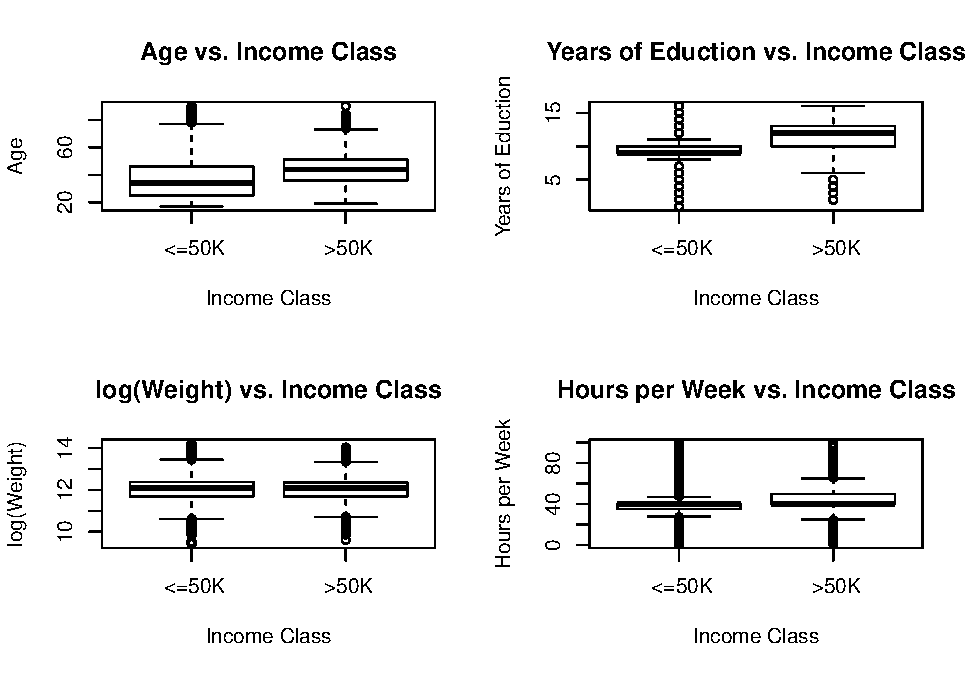
\includegraphics{post1_files/figure-latex/numerical data distribution in two groups-1.pdf}

\begin{Shaded}
\begin{Highlighting}[]
\KeywordTok{par}\NormalTok{(}\DataTypeTok{mfrow=}\KeywordTok{c}\NormalTok{(}\DecValTok{1}\NormalTok{,}\DecValTok{1}\NormalTok{))}
\end{Highlighting}
\end{Shaded}

numerical data distribution analysis:

\begin{enumerate}
\def\labelenumi{\arabic{enumi}.}
\item
  In group that income \textgreater{}50k, people are more likely to have
  higher average age, higher average education years and higher weekly
  work hours than whose income is \textless{}=50K.
\item
  Weight shows no difference in these two classes.
\end{enumerate}

\subsection{3. association rules of categorial
variables}\label{association-rules-of-categorial-variables}

\begin{Shaded}
\begin{Highlighting}[]
\KeywordTok{library}\NormalTok{(arules)}
\end{Highlighting}
\end{Shaded}

\begin{verbatim}
## Loading required package: Matrix
\end{verbatim}

\begin{verbatim}
## 
## Attaching package: 'arules'
\end{verbatim}

\begin{verbatim}
## The following objects are masked from 'package:base':
## 
##     abbreviate, write
\end{verbatim}

\begin{Shaded}
\begin{Highlighting}[]
\NormalTok{training<-training.data[,}\KeywordTok{c}\NormalTok{(}\DecValTok{2}\NormalTok{,}\DecValTok{4}\NormalTok{,}\DecValTok{6}\OperatorTok{:}\DecValTok{10}\NormalTok{,}\DecValTok{14}\NormalTok{,}\DecValTok{15}\NormalTok{)]}
\KeywordTok{summary}\NormalTok{(training)}
\end{Highlighting}
\end{Shaded}

\begin{verbatim}
##              workclass             education    
##   Private         :22696    HS-grad     :10501  
##   Self-emp-not-inc: 2541    Some-college: 7291  
##   Local-gov       : 2093    Bachelors   : 5354  
##   ?               : 1836    Masters     : 1723  
##   State-gov       : 1297    Assoc-voc   : 1382  
##   Self-emp-inc    : 1116    11th        : 1175  
##  (Other)          :  981   (Other)      : 5134  
##                 maritalstatus              occupation  
##   Divorced             : 4443    Prof-specialty :4140  
##   Married-AF-spouse    :   23    Craft-repair   :4099  
##   Married-civ-spouse   :14976    Exec-managerial:4066  
##   Married-spouse-absent:  418    Adm-clerical   :3769  
##   Never-married        :10682    Sales          :3650  
##   Separated            : 1025    Other-service  :3295  
##   Widowed              :  993   (Other)         :9541  
##           relationship                    race            sex       
##   Husband       :13193    Amer-Indian-Eskimo:  311    Female:10771  
##   Not-in-family : 8304    Asian-Pac-Islander: 1039    Male  :21789  
##   Other-relative:  981    Black             : 3124                  
##   Own-child     : 5068    Other             :  271                  
##   Unmarried     : 3446    White             :27815                  
##   Wife          : 1568                                              
##                                                                     
##         nativecountry      class      
##   United-States:29169    <=50K:24719  
##   Mexico       :  643    >50K : 7841  
##   ?            :  583                 
##   Philippines  :  198                 
##   Germany      :  137                 
##   Canada       :  121                 
##  (Other)       : 1709
\end{verbatim}

\begin{Shaded}
\begin{Highlighting}[]
\CommentTok{# use apriori rules to find association rules on people whose income class is >50K }
\NormalTok{rules <-}\StringTok{ }\KeywordTok{apriori}\NormalTok{(training,}
                 \DataTypeTok{control =} \KeywordTok{list}\NormalTok{(}\DataTypeTok{verbose=}\NormalTok{F),}
                 \DataTypeTok{parameter =} \KeywordTok{list}\NormalTok{(}\DataTypeTok{minlen=}\DecValTok{2}\NormalTok{, }\DataTypeTok{supp=}\FloatTok{0.005}\NormalTok{, }\DataTypeTok{conf=}\FloatTok{0.8}\NormalTok{),}
                 \DataTypeTok{appearance =} \KeywordTok{list}\NormalTok{(}\DataTypeTok{rhs=}\KeywordTok{c}\NormalTok{(}\StringTok{"class= >50K"}\NormalTok{),}
                                   \DataTypeTok{default=}\StringTok{"lhs"}\NormalTok{))}

\KeywordTok{inspect}\NormalTok{(}\KeywordTok{sort}\NormalTok{(rules, }\DataTypeTok{by=}\StringTok{"lift"}\NormalTok{, }\DataTypeTok{decreasing =} \OtherTok{TRUE}\NormalTok{)[}\DecValTok{1}\OperatorTok{:}\DecValTok{5}\NormalTok{])}
\end{Highlighting}
\end{Shaded}

\begin{verbatim}
##     lhs                                    rhs              support confidence     lift count
## [1] {workclass= Private,                                                                     
##      education= Masters,                                                                     
##      occupation= Exec-managerial,                                                            
##      relationship= Husband,                                                                  
##      nativecountry= United-States}      => {class= >50K} 0.00509828  0.9273743 3.850951   166
## [2] {workclass= Private,                                                                     
##      education= Masters,                                                                     
##      maritalstatus= Married-civ-spouse,                                                      
##      occupation= Exec-managerial,                                                            
##      relationship= Husband,                                                                  
##      nativecountry= United-States}      => {class= >50K} 0.00509828  0.9273743 3.850951   166
## [3] {workclass= Private,                                                                     
##      education= Masters,                                                                     
##      occupation= Exec-managerial,                                                            
##      relationship= Husband,                                                                  
##      sex= Male,                                                                              
##      nativecountry= United-States}      => {class= >50K} 0.00509828  0.9273743 3.850951   166
## [4] {workclass= Private,                                                                     
##      education= Masters,                                                                     
##      maritalstatus= Married-civ-spouse,                                                      
##      occupation= Exec-managerial,                                                            
##      sex= Male,                                                                              
##      nativecountry= United-States}      => {class= >50K} 0.00509828  0.9273743 3.850951   166
## [5] {workclass= Private,                                                                     
##      education= Masters,                                                                     
##      maritalstatus= Married-civ-spouse,                                                      
##      occupation= Exec-managerial,                                                            
##      relationship= Husband,                                                                  
##      sex= Male,                                                                              
##      nativecountry= United-States}      => {class= >50K} 0.00509828  0.9273743 3.850951   166
\end{verbatim}

\subsection{4. association rules
validation}\label{association-rules-validation}

\begin{Shaded}
\begin{Highlighting}[]
\CommentTok{# using test data and comfusion matrix to test the results }
\NormalTok{test<-test.data[,}\KeywordTok{c}\NormalTok{(}\DecValTok{2}\NormalTok{,}\DecValTok{4}\NormalTok{,}\DecValTok{6}\OperatorTok{:}\DecValTok{10}\NormalTok{,}\DecValTok{14}\NormalTok{,}\DecValTok{15}\NormalTok{)]}
\KeywordTok{summary}\NormalTok{(test)}
\end{Highlighting}
\end{Shaded}

\begin{verbatim}
##              workclass             education   
##   Private         :11209    HS-grad     :5283  
##   Self-emp-not-inc: 1321    Some-college:3587  
##   Local-gov       : 1043    Bachelors   :2670  
##   ?               :  963    Masters     : 934  
##   State-gov       :  683    Assoc-voc   : 679  
##   Self-emp-inc    :  579    11th        : 636  
##  (Other)          :  482   (Other)      :2491  
##                 maritalstatus             occupation  
##   Divorced             :2190    Prof-specialty :2032  
##   Married-AF-spouse    :  14    Exec-managerial:2020  
##   Married-civ-spouse   :7403    Craft-repair   :2013  
##   Married-spouse-absent: 210    Sales          :1854  
##   Never-married        :5433    Adm-clerical   :1841  
##   Separated            : 505    Other-service  :1628  
##   Widowed              : 525   (Other)         :4892  
##           relationship                   race            sex       
##   Husband       :6523    Amer-Indian-Eskimo:  159    Female: 5421  
##   Not-in-family :4278    Asian-Pac-Islander:  480    Male  :10859  
##   Other-relative: 525    Black             : 1560                  
##   Own-child     :2512    Other             :  135                  
##   Unmarried     :1679    White             :13946                  
##   Wife          : 763                                              
##                                                                    
##         nativecountry       class      
##   United-States:14661    <=50K.:12434  
##   Mexico       :  308    >50K. : 3846  
##   ?            :  274                  
##   Philippines  :   97                  
##   Puerto-Rico  :   70                  
##   Germany      :   69                  
##  (Other)       :  801
\end{verbatim}

\begin{Shaded}
\begin{Highlighting}[]
\NormalTok{test.rule1<-}\KeywordTok{subset}\NormalTok{(test, (workclass}\OperatorTok{==}\StringTok{' Private'}\NormalTok{) }\OperatorTok{&}\StringTok{ }\NormalTok{(education}\OperatorTok{==}\StringTok{' Masters'}\NormalTok{) }\OperatorTok{&}\StringTok{ }\NormalTok{(occupation}\OperatorTok{==}\StringTok{' Exec-managerial'}\NormalTok{) }\OperatorTok{&}\StringTok{ }\NormalTok{(relationship}\OperatorTok{==}\StringTok{' Husband'}\NormalTok{) }\OperatorTok{&}\StringTok{ }\NormalTok{(nativecountry}\OperatorTok{==}\StringTok{' United-States'}\NormalTok{))}
\NormalTok{accuracy.rules1=}\KeywordTok{nrow}\NormalTok{(}\KeywordTok{subset}\NormalTok{(test.rule1,class}\OperatorTok{==}\StringTok{' >50K.'}\NormalTok{))}\OperatorTok{/}\KeywordTok{nrow}\NormalTok{(test.rule1)}

\NormalTok{test.rule2<-}\KeywordTok{subset}\NormalTok{(test,workclass}\OperatorTok{==}\StringTok{' Private'} \OperatorTok{&}\StringTok{ }\NormalTok{education}\OperatorTok{==}\StringTok{' Masters'} \OperatorTok{&}\StringTok{ }\NormalTok{maritalstatus}\OperatorTok{==}\StringTok{' Married-civ-spouse'} \OperatorTok{&}\StringTok{ }\NormalTok{occupation}\OperatorTok{==}\StringTok{' Exec-managerial'} \OperatorTok{&}\StringTok{ }\NormalTok{relationship}\OperatorTok{==}\StringTok{' Husband'} \OperatorTok{&}\StringTok{ }\NormalTok{nativecountry}\OperatorTok{==}\StringTok{' United-States'}\NormalTok{)}
\NormalTok{accuracy.rules2=}\KeywordTok{nrow}\NormalTok{(}\KeywordTok{subset}\NormalTok{(test.rule2,class}\OperatorTok{==}\StringTok{' >50K.'}\NormalTok{))}\OperatorTok{/}\KeywordTok{nrow}\NormalTok{(test.rule2)}

\NormalTok{test.rule3<-}\KeywordTok{subset}\NormalTok{(test,workclass}\OperatorTok{==}\StringTok{' Private'} \OperatorTok{&}\StringTok{ }\NormalTok{education}\OperatorTok{==}\StringTok{' Masters'} \OperatorTok{&}\StringTok{ }\NormalTok{occupation}\OperatorTok{==}\StringTok{' Exec-managerial'} \OperatorTok{&}\StringTok{ }\NormalTok{relationship}\OperatorTok{==}\StringTok{' Husband'} \OperatorTok{&}\StringTok{ }\NormalTok{sex}\OperatorTok{==}\StringTok{' Male'}\NormalTok{)}
\NormalTok{accuracy.rules3=}\KeywordTok{nrow}\NormalTok{(}\KeywordTok{subset}\NormalTok{(test.rule3,class}\OperatorTok{==}\StringTok{' >50K.'}\NormalTok{))}\OperatorTok{/}\KeywordTok{nrow}\NormalTok{(test.rule3)}


\NormalTok{test.rule4<-}\KeywordTok{subset}\NormalTok{(test,workclass}\OperatorTok{==}\StringTok{' Private'} \OperatorTok{&}\StringTok{ }\NormalTok{education}\OperatorTok{==}\StringTok{' Masters'} \OperatorTok{&}\StringTok{ }\NormalTok{maritalstatus}\OperatorTok{==}\StringTok{' Married-civ-spouse'} \OperatorTok{&}\StringTok{ }\NormalTok{occupation}\OperatorTok{==}\StringTok{' Exec-managerial'} \OperatorTok{&}\StringTok{ }\NormalTok{sex}\OperatorTok{==}\StringTok{' Male'} \OperatorTok{&}\StringTok{ }\NormalTok{nativecountry}\OperatorTok{==}\StringTok{' United-States'}\NormalTok{)}
\NormalTok{accuracy.rules4=}\KeywordTok{nrow}\NormalTok{(}\KeywordTok{subset}\NormalTok{(test.rule4,class}\OperatorTok{==}\StringTok{' >50K.'}\NormalTok{))}\OperatorTok{/}\KeywordTok{nrow}\NormalTok{(test.rule4)}


\NormalTok{test.rule5<-}\KeywordTok{subset}\NormalTok{(test,workclass}\OperatorTok{==}\StringTok{' Private'} \OperatorTok{&}\StringTok{ }\NormalTok{education}\OperatorTok{==}\StringTok{' Masters'} \OperatorTok{&}\StringTok{ }\NormalTok{maritalstatus}\OperatorTok{==}\StringTok{' Married-civ-spouse'} \OperatorTok{&}\StringTok{ }\NormalTok{occupation}\OperatorTok{==}\StringTok{' Exec-managerial'} \OperatorTok{&}\StringTok{ }\NormalTok{relationship}\OperatorTok{==}\StringTok{' Husband'} \OperatorTok{&}\StringTok{ }\NormalTok{sex}\OperatorTok{==}\StringTok{' Male'} \OperatorTok{&}\StringTok{ }\NormalTok{nativecountry}\OperatorTok{==}\StringTok{' United-States'}\NormalTok{)}
\NormalTok{accuracy.rules5=}\KeywordTok{nrow}\NormalTok{(}\KeywordTok{subset}\NormalTok{(test.rule5,class}\OperatorTok{==}\StringTok{' >50K.'}\NormalTok{))}\OperatorTok{/}\KeywordTok{nrow}\NormalTok{(test.rule5)}

\KeywordTok{paste}\NormalTok{(}\StringTok{'accuracy of association rule1,rule2,rule3,rule4 and rule5 are:'}\NormalTok{,}\KeywordTok{round}\NormalTok{(accuracy.rules1,}\DecValTok{3}\NormalTok{),}\KeywordTok{round}\NormalTok{(accuracy.rules2,}\DecValTok{3}\NormalTok{),}\KeywordTok{round}\NormalTok{(accuracy.rules3,}\DecValTok{3}\NormalTok{), }\KeywordTok{round}\NormalTok{(accuracy.rules4,}\DecValTok{3}\NormalTok{), }\KeywordTok{round}\NormalTok{(accuracy.rules5,}\DecValTok{3}\NormalTok{))}
\end{Highlighting}
\end{Shaded}

\begin{verbatim}
## [1] "accuracy of association rule1,rule2,rule3,rule4 and rule5 are: 0.909 0.909 0.885 0.909 0.909"
\end{verbatim}

\subsection{5. conclusions}\label{conclusions}

\begin{Shaded}
\begin{Highlighting}[]
\CommentTok{#1. numerical statistic analysis showed that people have higher average age, higher average education years and higher weekly work hours are more likely to have income >50K. }

\CommentTok{#2. association rules listed in this project showed good accuracies: rule1(91%),rule2(91%),rule3(89%),rule4(91%),rule5(91%). }

\CommentTok{#3. association rules showed that people who have master degrees, work privately married male with an Exec-managerial occupation have large possibilities(>80%) to have salaries more than 50,000. }
\end{Highlighting}
\end{Shaded}


\end{document}
